\documentclass[11pt,letterpaper]{article}
\usepackage[utf8]{inputenc}
\usepackage[margin=1in]{geometry}
\usepackage[margin=1cm]{caption}
\usepackage{amsmath}
\usepackage{amsfonts}
\usepackage{amssymb}
\usepackage{amsthm}
\usepackage{verbatim}
\usepackage{graphicx}
\usepackage{siunitx}
\usepackage{animate}
% No paragraph tabs
\setlength{\parindent}{0pt}

% Define commands that will be widely used.
\newcommand{\br}{\ \\}
\newcommand{\tab}{\hspace*{2em}}

\title{Analog circuits}
\author{Isaac Domagalski}
\date{February 10, 2014}

\begin{document}
\maketitle

\begin{abstract}
    In this lab, an FM demodulator was constructed. Based on the components
    used, the RLC bandpass in the demodulator had a resonance frequency of 
    \SI{1.07}{\mega\hertz}, and a bandwidth of \SI{219}{\kilo\hertz}. The RC
    low-pass filter used to smooth the signal had a rolloff point at
    \SI{106}{\kilo\hertz}. The output of the FM demodulator was then plugged
    into a common-emitter amplifier, where the ratio of $R_C$ to $R_E$ was 2.32.
    The FM demodulator was able to successfully extract signals modulated in FM
    with a \SI{1.045}{\mega\hertz} carrier frequency. Additionally, the speed of
    propagation of signals in a BNC cable was measured to be
    \SI{1.9e8}{\meter/\second}.
\end{abstract}

\section{Introduction}

Frequency demodulation and amplification contain many important concepts in the
basics of analog circuits. A frequency-modulated (FM) signal has the
mathematical form \cite{FMWikipedia}
\begin{equation}
    y\left(t\right) = A_c \cos\left(2\pi f_c t +
    2 \pi f_{\Delta} \int_0^t x_m\left(\tau\right) d\tau
    \right)
\end{equation}
where $A_c$ is the carrier amplitude, $f_c$ is the carrier frequency,
$f_{\Delta}$ is the maximum frequency deviation, and $x_m$ is the signal being
transmitted. Many radio stations are broadcast in FM, and electronic circuits
that are able to convert an FM signal to the signal encoded in the FM, such as
FM demodulators, are needed. While FM demodulators are useful for extracting
signals encoded in FM, in order for signals to be audible, they must go through
an amplifier. One common amplifier design, which will be discussed in detail
later, is the common-emitter amplifier. The common-emitter amplifier uses a
transistor circuit to amplify signals, where the gain is the ratio of the
collector resistor to the emitter resistor.
\\

Signals often must be sent from one physical location to another. In order to do
this, a transmission line must be used. It is possible for one to point to many
different types of cables and say that ``this is a transmission line,'' but the
simplest understanding of a transmission line is that it is a cable that
transmits electrical energy from one location to another. One very useful
property of transmission lines is that their impedance does not depend on the
length of the cable. While transmission lines are very useful, one possible
problem with them is that reflections on the cable can occur and distort a
signal. The amount of wave that gets reflected in a transmission line is
governed by the reflection coefficient \cite{AstroBaki}
\begin{equation}
    \Gamma = \frac{Z_{load} - Z_0}{Z_{load} + Z_0}
    \label{reflection}
\end{equation}
where $Z_{load}$ is the impedance of whatever the cable is plugged into and
$Z_0$ is the impedance of the cable itself. There is also a related coefficient
called the transmission coefficient, where $T = 1 + \Gamma$. One thing that can
be deduced from \eqref{reflection} is that if one wants to prevent reflections
in a transmission line from occurring, then one must attach a load that is equal
to the impedance of the cable being used to transmit a signal. Typical BNC and
SMA cables have impedances of about \SI{50}{\ohm} and termination resistors for
these cables are fairly common.

\section{The FM Demodulator}

\begin{figure}
    \centering
    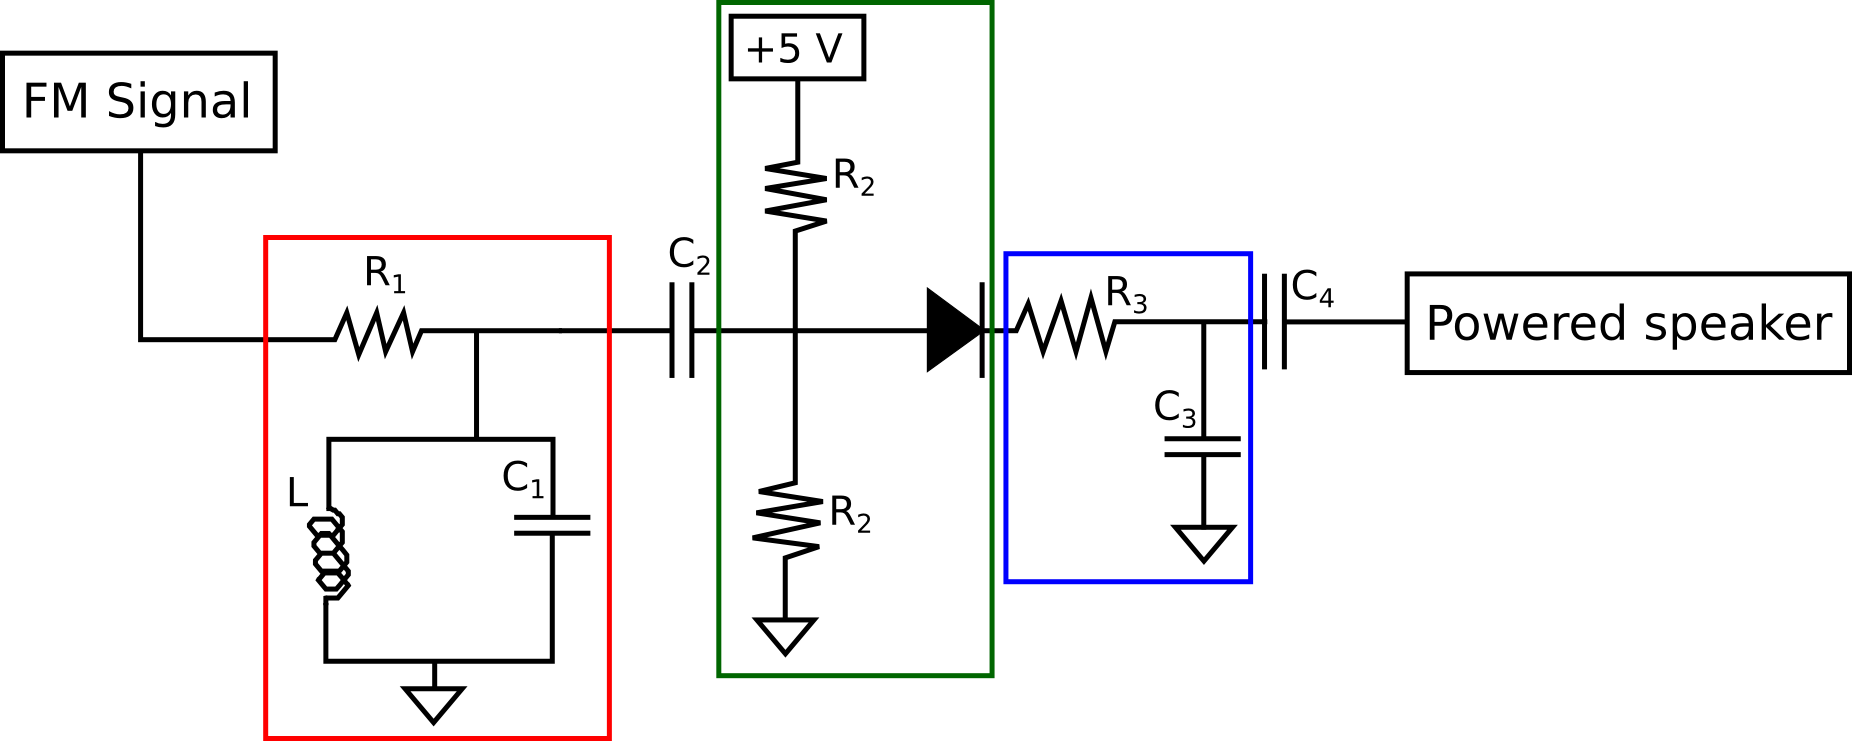
\includegraphics[width=\textwidth]{figures/demod.png}
    \caption{Circuit diagram of the FM demodulator. Different units in the
    circuit are highlighted with the colored boxes.}
    \label{demod}
\end{figure}

The goal of the FM demodulator is to extract an signal from an FM radio wave.
The FM demodulator used can be seen in Figure~\ref{demod}. First, an frequency
modulated signal is provided by a function generator and an audio player. The
signal travels though an RLC bandpass filter, which can be seen in the red box,
which converts an FM signal to an AM signal. After that, a DC offset is applied
to a signal before going through a diode, which is used to clip the bottom of
the signal. Finally, the signal travels through a low-pass filter, denoted by
the blue box, which removes high frequency oscillations from the signal, which
allows the encoded signal to pass through. Finally, the signal runs though the
capacitor $C_4$, which removes any remaining DC bias from the signal. After
that, the signal is fed into either a speaker or an amplifier. In this lab, the
carrier frequency of the FM signal is \SI{1.045}{\mega\hertz}.

\subsection{The RLC Filter}

\begin{figure}
    \centering
    \begin{minipage}[t]{0.45\textwidth}
        \centering
        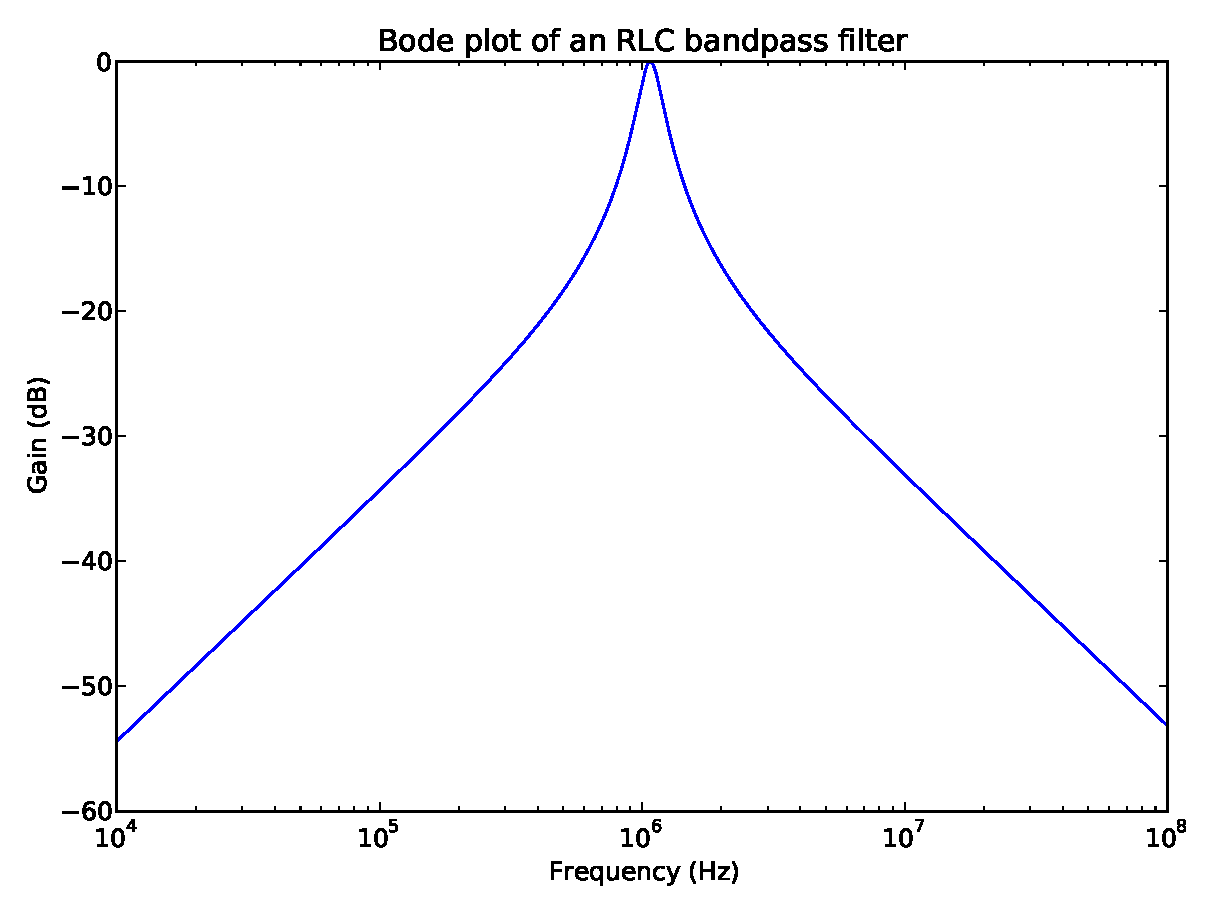
\includegraphics[width=\textwidth]{figures/bandpass.pdf}
    \end{minipage}
    \hspace{0.5cm}
    \begin{minipage}[t]{0.45\textwidth}
        \centering
        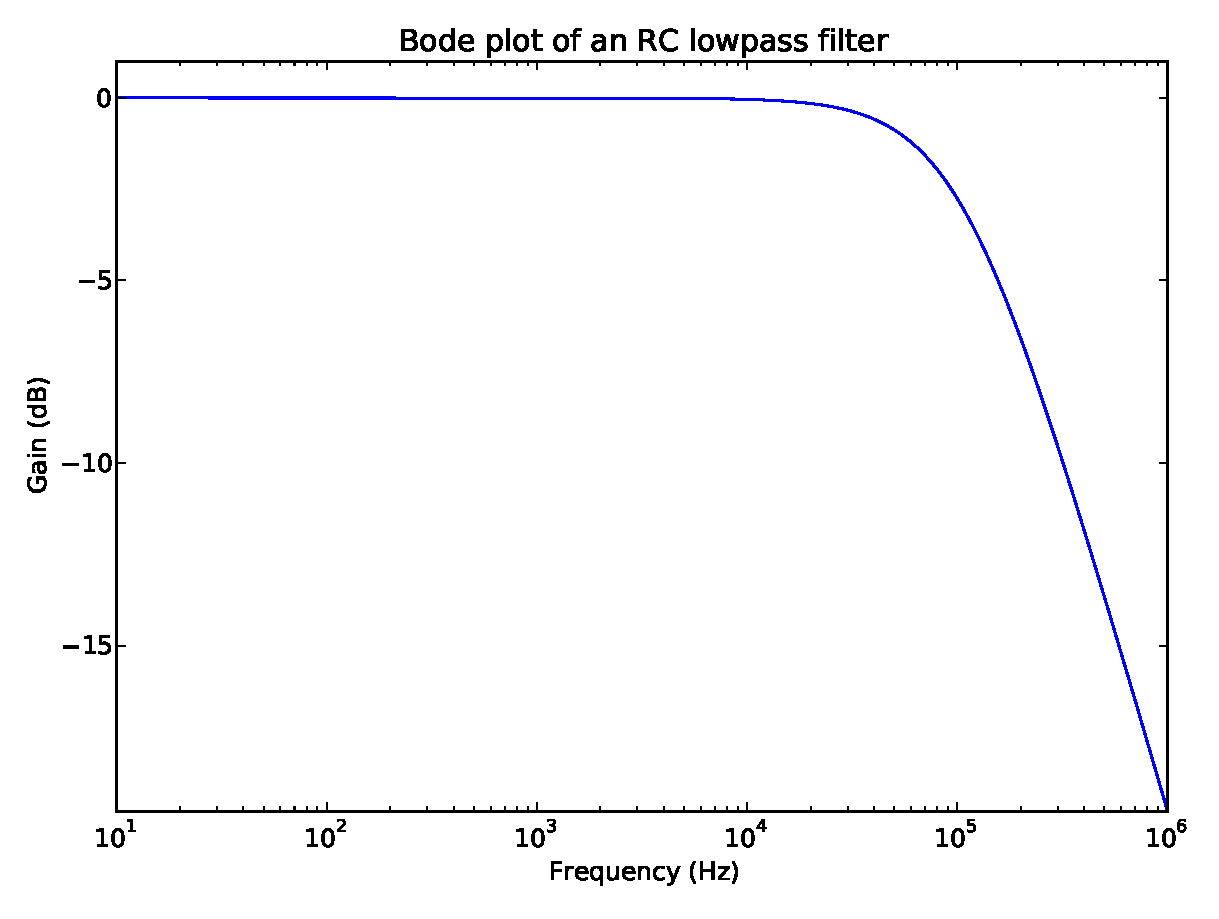
\includegraphics[width=\textwidth]{figures/lowpass.pdf}
    \end{minipage}
    \caption{Gain can be expressed in decibels using the formula
        $20\log_{10}\left|\dfrac{V_{out}}{V_{in}}\right|$.}
    \label{bandpass}
\end{figure}

The RLC filter is the part of Figure~\ref{demod} that is enclosed in the red
box and the purpose of the filter was to convert an FM signal into an AM signal.
The response of the RLC filter can be computed using the voltage divider
equation as $\left|\dfrac{Z}{Z+R}\right|$, where $Z$ is the equivalent
impedance of the LC parallel circuit. This evaluates to
\begin{equation}
    \left|\frac{V_{out}}{V_{in}}\right| = 
    \frac{\omega L}{\sqrt{R^2\left(\omega^2 LC - 1\right)^2 + \omega^2 L^2}}
    \label{rlc_filter}
\end{equation}
where $\omega = 2\pi f$. It can be seen from inspection that \eqref{rlc_filter}
has a maximum value of 1 at $f_0 = \dfrac{1}{2\pi\sqrt{LC}}$, which is the
resonance frequency of the circuit. The transfer function for the RLC bandpass
can be seen in Figure~\ref{bandpass}. Since the RLC circuit is a bandpass, there
are two roll-off points where the transfer function goes below $\SI{-3}{dB}$,
which are located at
\begin{equation}
    f_{\SI{-3}{dB}} = \frac{1}{2\pi}\sqrt{
        \frac{1}{LC} + 
        \frac{1}{2R^2C^2} \pm
        \sqrt{
            \frac{1}{R^2C^3L} + 
            \frac{1}{4R^4C^4}
        }
    }
    \label{rlc_rolloff}
\end{equation}

The values of $R$, $L$, and $C$ are determined by the specifications of the
bandpass. The goal was to tune the LC parallel circuit it \SI{1}{\mega \hertz}.
Since the only inductors available in the lab were \SI{1}{\micro \henry}, the
capacitor required for the desired resonance frequency is about
\SI{25.3}{\nano \farad}. Since the capacitor with the value closest to what was
required for the \SI{1}{\mega\hertz} resonance was \SI{22}{\pico\farad}, the RLC
circuit theoretically had a resonance of \SI{1.07}{\mega\hertz}. The value of
$R$ was chosen by using a bandpass of $\Delta f_{\SI{-3}{dB}} =
\SI{200}{\kilo\hertz}$ and using the appropriate $Q$ factor to match that
condition. Using the fact that
$Q = \omega_0 RC = \dfrac{f_0}{\Delta f_{\SI{-3}{dB}}}$
and the values of $L$ and $C$, the best resistor for the RLC circuit was
determined to be a \SI{36}{\ohm} resistor. The resistor chosen for the circuit
was a \SI{33}{\ohm}. Using the actual values of $R$, $L$, and $C$ used in the
bandpass filter, both \eqref{rlc_rolloff} and the $Q$ factor equation give the
same prediction that $\Delta f_{\SI{-3}{dB}} = \SI{219}{\kilo\hertz}$.

\subsection{The Envelope Detector}

\begin{figure}
    \centering
    \animategraphics[autoplay,loop,width=0.6\textwidth]{10}{am/am-wave-}{00}{19}
    \caption{Example of an amplitude-modulated wave (blue) with its envelope
    (red).}
    \label{amwave}
\end{figure}

The green and blue boxes in Figure~\ref{demod} form an envelope detector. The
goal of an envelope detector is to extract a signal from an amplitude-modulated
(AM) wave. This can be seen in Figure~\ref{amwave}, where the AM signal is in
blue and the envelope, which is the signal that is getting extracted, is the red
curve. The envelope detector consists of two main parts. The first is the diode,
which is in the green box, and the second is the low-pass filter in the blue
box.\\

The use of the diode in the envelope detector is pretty straightforward. Since
current can only flow one way though a diode, the diode cuts off the bottom half
of the signal. This is desirable, as the envelope to extract is only on the top
half of the signal anyways. The part of Figure~\ref{demod} enclosed in the green
box involving a voltage source and the resistors $R_2$ (\SI{150}{\ohm} resistors
were used in the circuit) adds a current bias. This is useful, because there
needs to be a large enough voltage drop across the diode in order for current to
flow. Typically, there needs to be a \SI{0.6}{\volt} voltage drop across the
diode in order for it to conduct properly.\\

The signal that makes it through the diode must then go through a low-pass
filter, which can be seen in the blue box in Figure~\ref{demod}. The purpose of
the low-pass filter is to remove high-frequency oscillations from the signal it
gets in order to smooth out the envelope. The components used for the low-pass
filter were a \SI{100}{\ohm} resistor for $R_3$ and a \SI{10}{\nano\farad}
capacitor for $C_3$. This gives a rolloff frequency of \SI{106}{\kilo\hertz},
which will make sure that the \SI{1.045}{\mega\hertz} carrier frequency is
absent from the output signal.

% Present a circuit diagram of an FM radio receiver, highlighting blocks of
% components that act as a unit to perform some action (filtering, biasing,
% etc.)
% 
% Describe in the text the overall design of the FM receiver, with subsections
% for each functional block, listing salient features of each (e.g. the -3dB
% point of a filter, the voltage biased to, etc.). Present it as if you invented
% it, and were writing the seminal paper that will enable others to use this
% design.
% 
% Using your new understanding of impedances, plot the expected output of the LC
% filter in your FM receiver as a function of frequency, f = w /2\pi. Mark the
% location, in frequency, of the transmission band used in the lab, and explain
% the rational behind its placement on the LC response curve (e.g. if our
% station is at 1.045 MHz, why is your LC tuned to 1.0 MHz?)
% 
% Finally, also plot, as a function of frequency, the bandpass of the final
% filter that defines the band of the output audio signal. Describe (and maybe
% plot) the rationale for selecting the filter that you did.

\section{The Common-Emitter Amplifier}

\begin{figure}
    \centering
    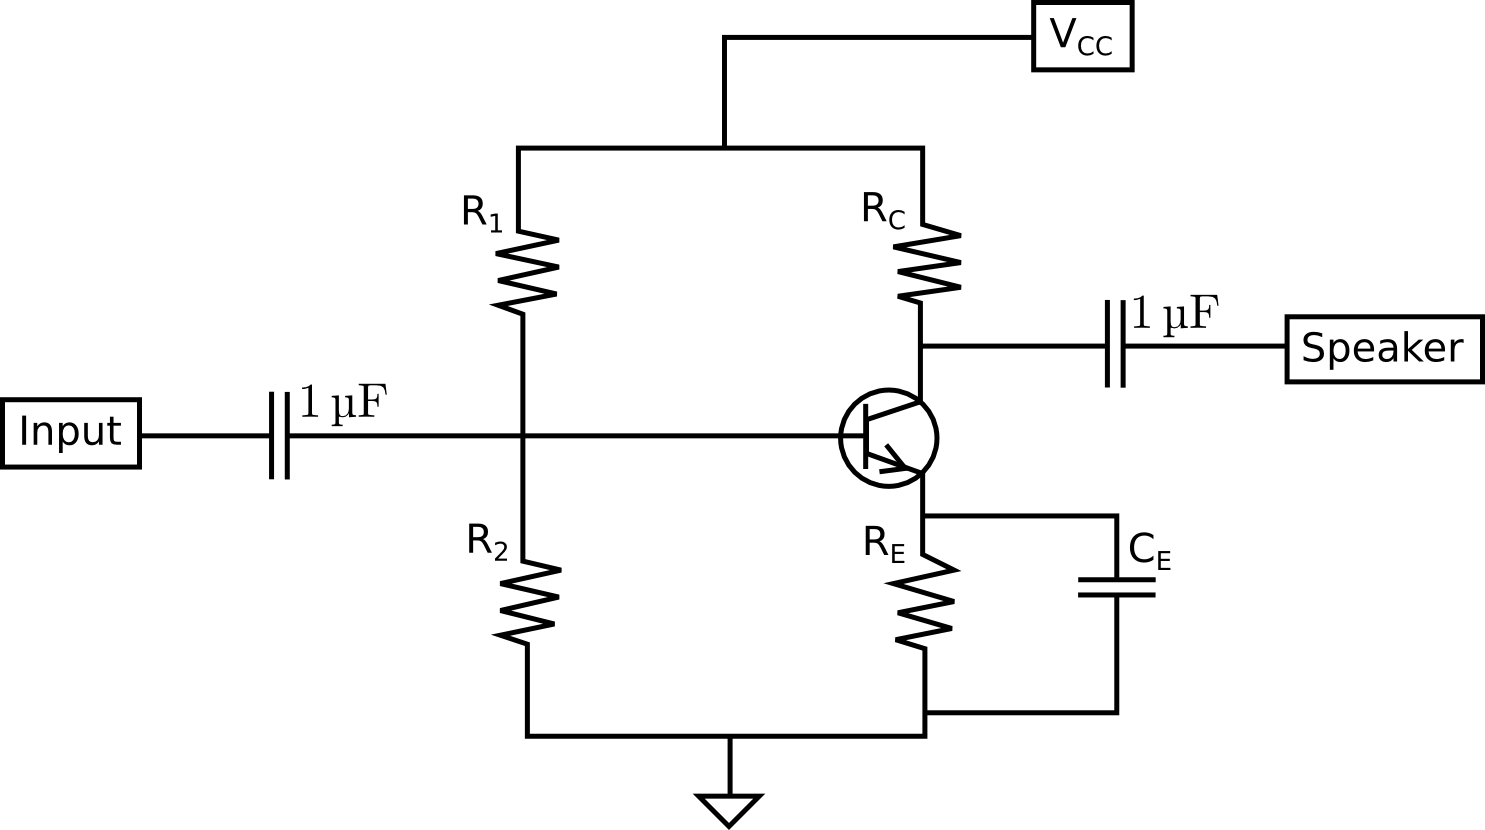
\includegraphics[width=\textwidth]{figures/amplifier.png}
    \caption{Circuit diagram of the common-emitter amplifier.}
    \label{amplifier}
\end{figure}

\begin{figure}
    \centering
    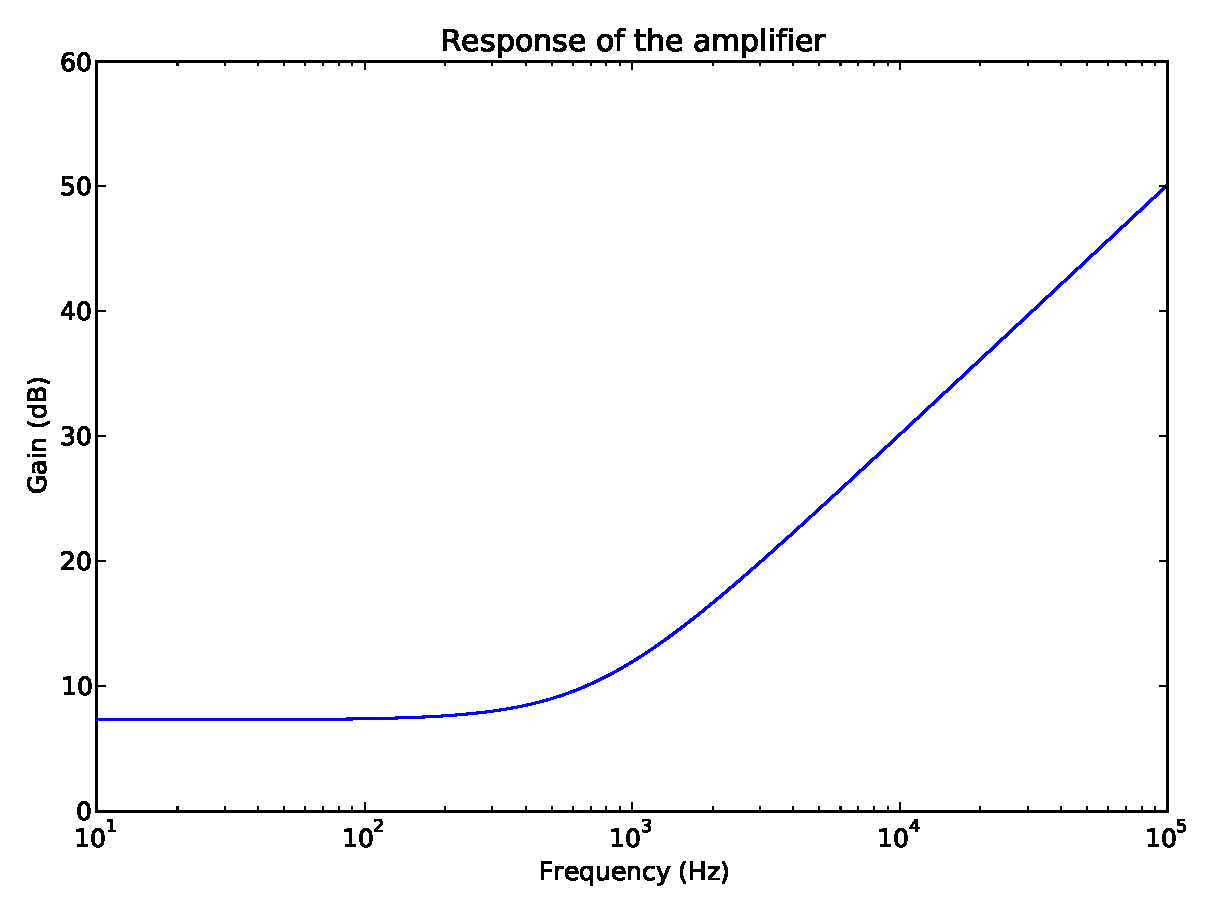
\includegraphics[width=0.7\textwidth]{figures/ampgain.pdf}
    \caption{The gain of the amplifier increases as the frequency increases.}
    \label{ampgainplot}
\end{figure}

\subsection{Amplifier Design}

The signal coming out of the FM demodulator is very low, so in order to make it
audible, it must be amplified. The amplifier used to amplify the signal before
it went to the speaker can be seen in Figure~\ref{amplifier}. The gain of the
amplifier is specified by $|R_C / Z_E|$, where
$Z_E^{-1} = R_E^{-1} + X_{C_E}^{-1}$, and $X_{C_E} = \dfrac{1}{jwC_E}$. This
evaluates to the gain of the amplifier being
\begin{equation}
    g = \frac{R_C}{R_E} \sqrt{1 + \omega^2 R_E^2 C_E^2}
    \label{ampgain}
\end{equation}
where $\omega = 2\pi f$. This gain is useful for amplifying high-frequency
signals and is approximately linear for large frequencies. In order to achieve a
gain of about 2 when there is no capacitor, $R_C$ was set to \SI{510}{\ohm} and
$R_C$ was set to \SI{220}{\ohm}. Due to what was available in the lab, a 
\SI{1}{\micro\farad} capacitor was used for $C_E$. Without the capacitor, the
gain of the amplifier was 2.32, which is \SI{7.3}{\deci\bel}. The response of
the amplifier, in decibels, can be seen in Figure~\ref{ampgainplot}. At low
frequencies, the response is flat, but starts to increase at frequencies of
\SI{500}{\hertz}. This makes the amplifier sort-of suitable for music, where
notes are typically between \SI{30}{Hz} and \SI{4}{\kilo\hertz}.\\

The resistors $R_1$ and $R_2$ do not do the gain, but they are important for the
amplifier, as they set the bias voltage at the base. The resistors $R_1$ and
$R_2$ form a voltage divider, which sets the base voltage bias at
$\dfrac{R_2}{R_1 + R_2} V_{CC}$, where $V_{CC}$ is typically set at
\SI{5}{\volt}. Since $V_{BE}$ was measured to be \SI{0.73}{\volt} for the
transistor used in the amplifier, the base voltage was decided to be given a
bias of about \SI{1}{\volt}. This was done by setting $R_1$ to \SI{3900}{\ohm}
and $R_2$ to \SI{996}{\ohm}. $R_2$ was created from a series of resistors as no
\SI{1}{\kilo\ohm} resistors seemed to be available in the lab. Using these
resistor values, the base of the transistor was biased to \SI{1.01}{\volt} with
$V_{CC}$ set at \SI{5}{\volt}. The maximum operating amplitude for a 
\SI{10}{\kilo\hertz} wave was measured to be \SI{30}{\milli\volt}. Increasing
$V_{CC}$ up to \SI{31.5}{\volt} increased the maximum operating amplitude at 
\SI{10}{\kilo\hertz} up to \SI{800}{\milli\volt}.

\subsection{Connection the amplifier to transmission lines}

\begin{figure}
    \centering
    \begin{minipage}[t]{0.45\textwidth}
        \centering
        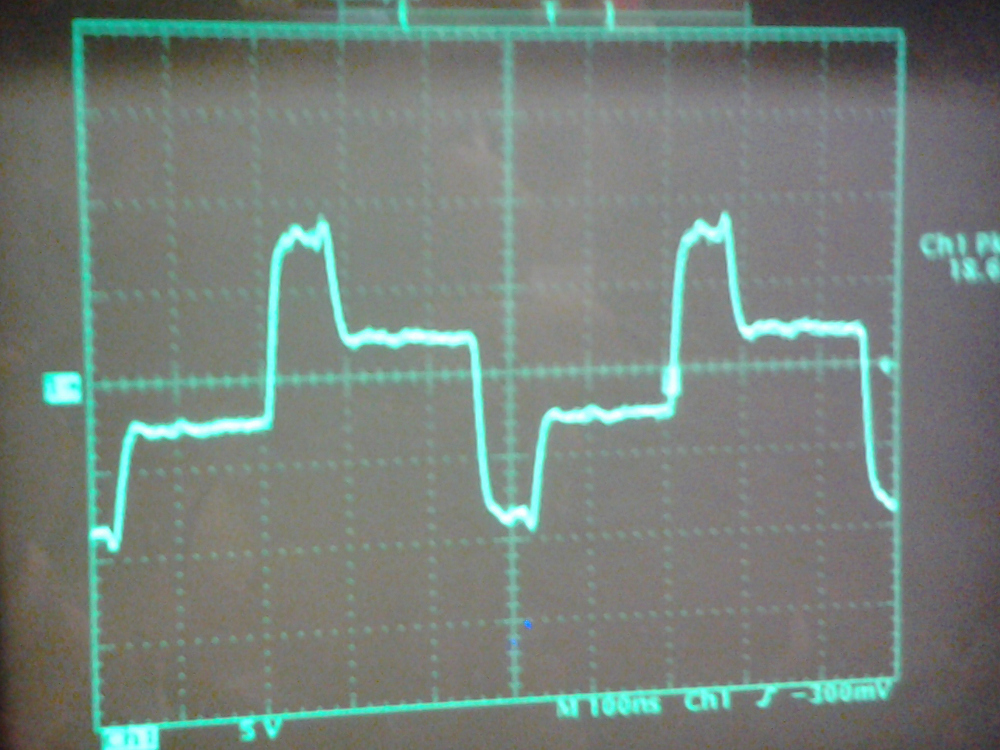
\includegraphics[width=\textwidth]{figures/reflection.jpg}
        \caption{Reflected waves on a long BNC cable. The end of the cable is
            shorted.}
        \label{reflected}
    \end{minipage}
    \hspace{0.5cm}
    \begin{minipage}[t]{0.45\textwidth}
        \centering
        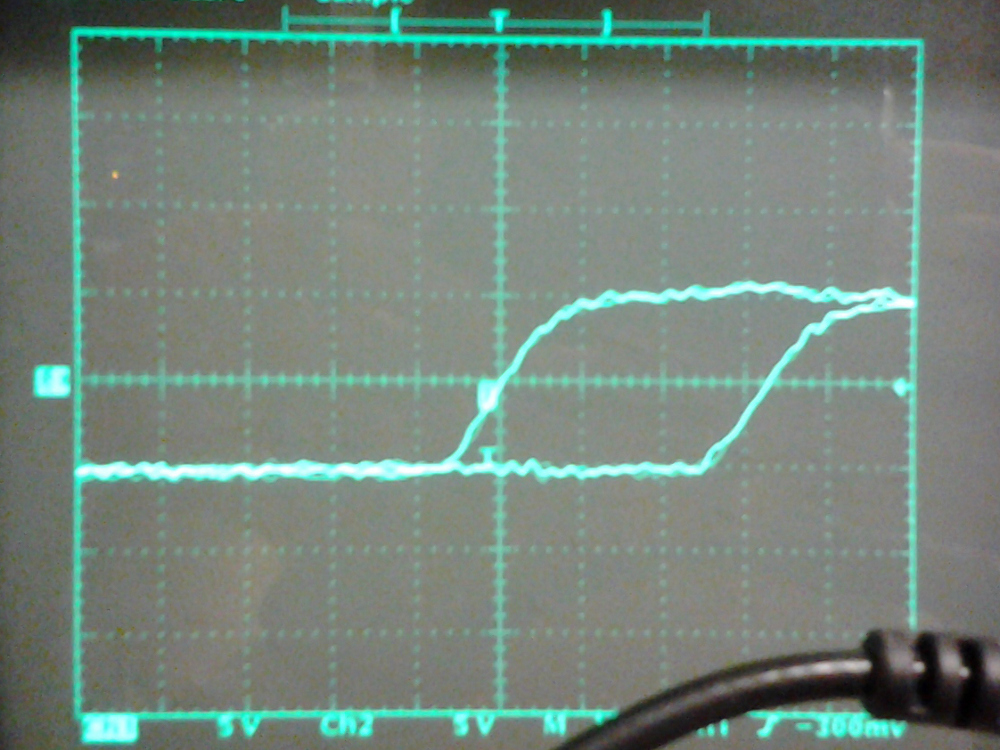
\includegraphics[width=\textwidth]{figures/speed.jpg}
        \caption{Directly measuring the time it takes for a signal to propagate
            along the BNC cable.}
        \label{speed}
    \end{minipage}
\end{figure}

Suppose that the amplifier was connected to a very long BNC cable before it was
connected to a speaker. When transmission lines are long, reflections of waves
along them become more noticeable. In order to deal with this, transmission
cables need to be terminated properly. According to \eqref{reflection}, if the
load impedance is equal to the impedance of the cable, then there will be no
reflections along the cable. Audio speakers typically have impedances of 
\SI{8}{\ohm}, so adding a \SI{42}{\ohm} resistor in series with the speakers
should properly terminate the cable so that no waves get reflected.\\

The effect of reflections can be seen in Figure~\ref{reflected}. The cable used
was made by combining several BNC cables until there was about 6.22 meters worth
of cable. Since the end of the cable is shorted, then according to
\eqref{reflection}, $\Gamma = -1$, which means that a wave of equal magnitude,
but inverted gets reflected back down the BNC cable. However, due to the length
of the cable, the reflected wave does not align with the incident wave. There is
a time delay due to the amount of time it takes for a signal to travel down a
cable. This time delay does not depend on frequency and only depends on the
length of the cable.\\

The following setup was employed to measure the speed of propagation along the
BNC cable. First, a properly terminated cable was plugged so that one end was in
Channel 1 of the scope and the other end, 6.22 feet of cable in between, was
plugged into Channel 2 of the scope. The input waveform was a square wave. It
was found that there was a delay of \SI{32}{\nano\second} between the two
channels, which can be seen in Figure~\ref{speed}. Based on these measurements,
the speed of propagation along the BNC cable is approximately 
\SI{1.9e8}{\meter /\second}. Since the speed of light in a material is
\begin{equation}
    v = \frac{1}{\sqrt{\epsilon\mu}} \approx
        \frac{1}{\sqrt{\epsilon_r\epsilon_0\mu_0}}
\end{equation}
it can be concluded that the relative permittivity, $\epsilon_r$, for the BNC
cable is about 2.4.

% Add a section describing your speaker amplifier, including a circuit diagram,
% and describing how it functions (and what the various functional parts are).
% I'll be looking for a description of how the base and collector voltages are
% set, and why they needed to be set where they are.
% 
% Specify the input and output impedance of your circuit at audio (~10 kHz)
% frequencies.
% 
% Suppose your speaker amplifier connects to a speaker at the end of a long run
% of wire. Given the amplifier circuit that you built, what impedance cable to
% you recommend, and how would you terminate it (incorporating an 8-Ohm speaker)
% to avoid reflections? For now, don't worry, unless you want to, about
% maximizing the current through the speaker (to make it LOUD).

\section{Noise}

\begin{figure}
    \centering
    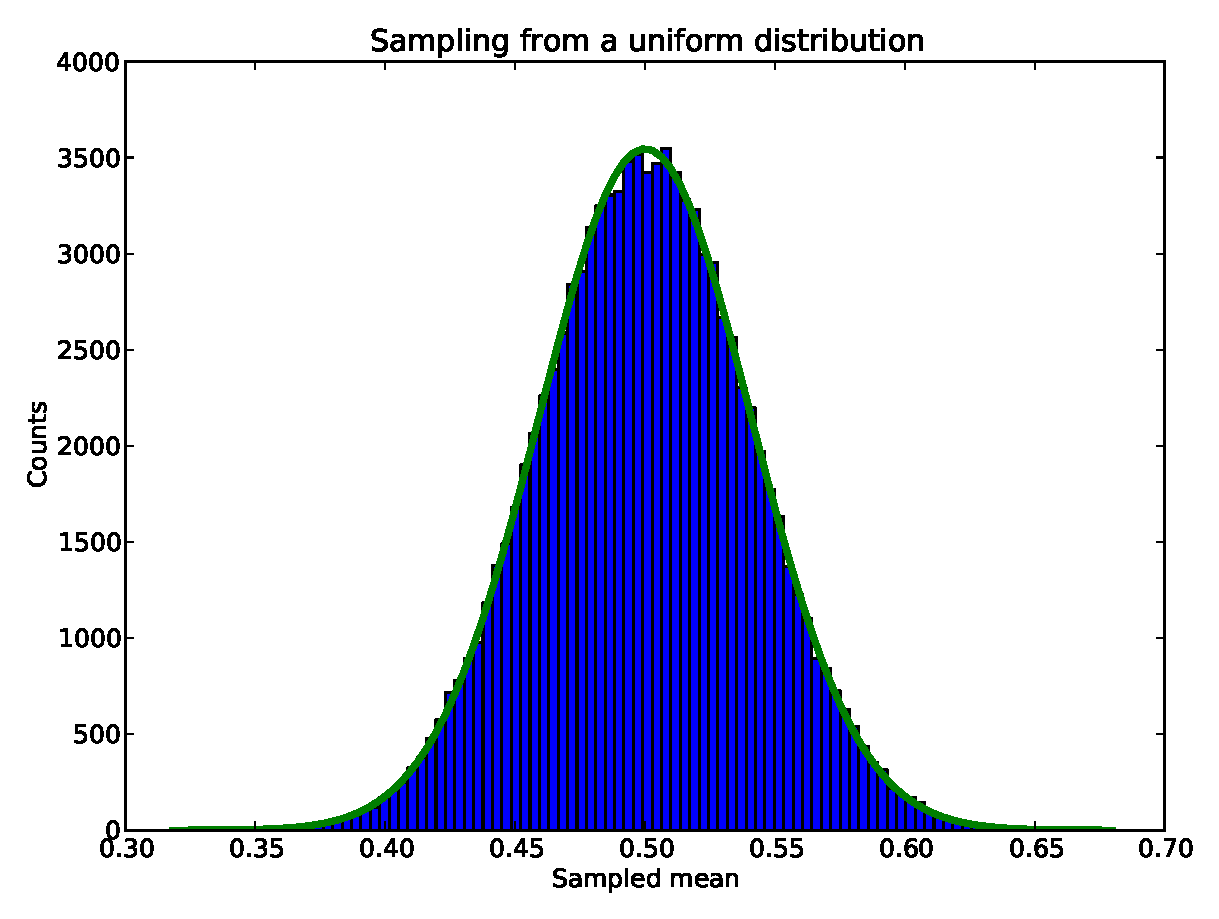
\includegraphics[width=0.7\textwidth]{figures/cl_uniform.pdf}
    \caption{Demonstration of the central limit theorem. The distribution that
    the sampled means were taken from was a uniform distribution from 0 to 1.
    The sample size for each mean was 50 and 100,000 samples were taken. The
    green line is a Gaussian curve where the mean is the expected mean of a
    uniform distribution and the standard deviation is the expected standard
    deviation divided by the square root of the sample size.}
    \label{cl_thm}
\end{figure}

\begin{figure}
    \centering
    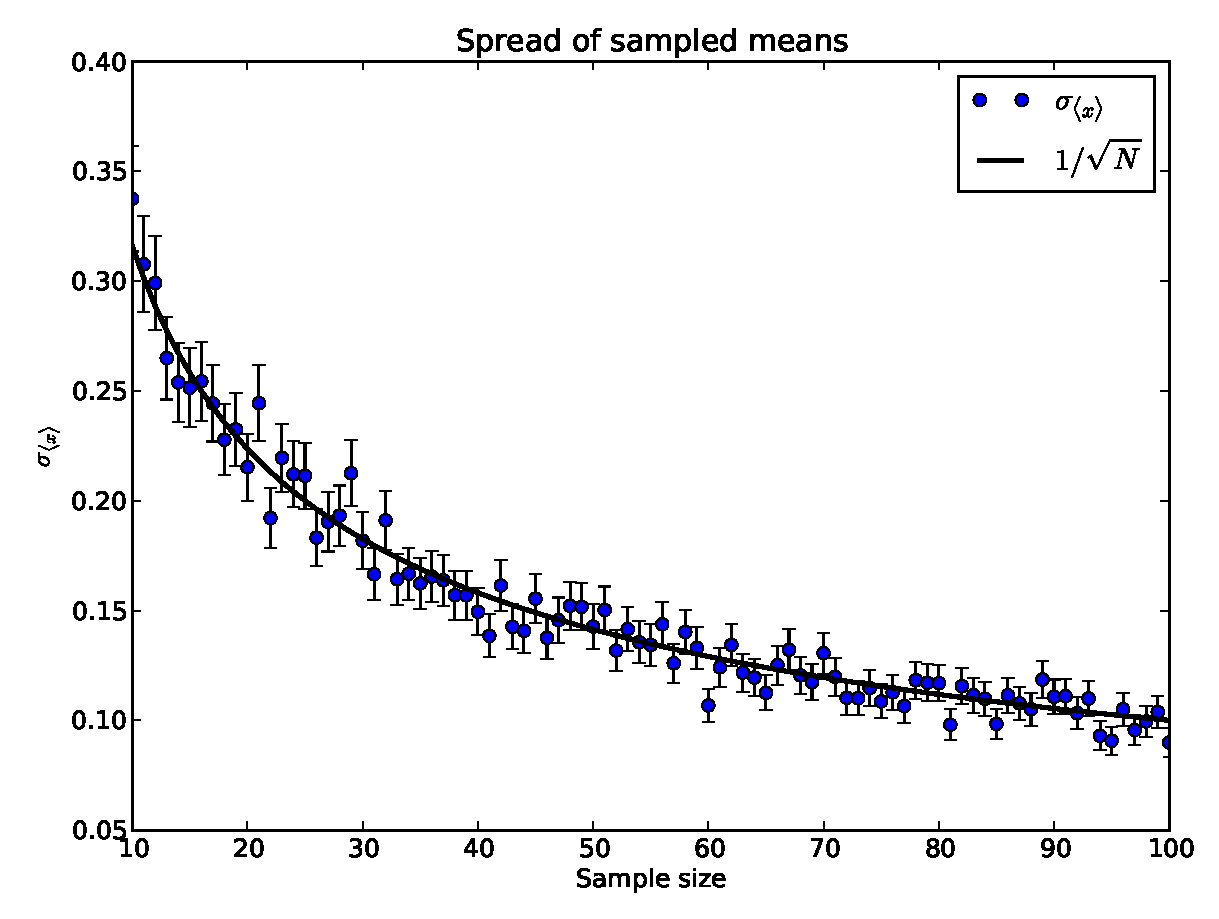
\includegraphics[width=0.7\textwidth]{figures/root_n.pdf}
    \caption{The standard deviation of a mean drops as $1 / \sqrt{N}$. In this
    plot, the sample size used to sample the mean of a standard normal
    distribution is varied. The standard deviation of the sampled means is
    calculated from 100 sampled means for every sample size.}
    \label{root_n}
\end{figure}

It is impossible to build a circuit without noise. The thermal motion of
electrons produces noise, known as Johnson-Nyquist noise, which produces noise
power of $P = 4 k_B T B$ \cite{JNWikipedia}, where $K_B$ is Boltzmann's
constant, $T$ is the temperature, and $B$ is that bandwidth of the system. If
one wanted to find the noise of the amplifier in Figure~\ref{amplifier}, then
one would only need to calculate or measure the operating bandwidth of the
circuit. In Figure~\ref{amplifier}, $R_2$ and the \SI{1}{\micro\farad} capacitor
form a high-pass filter. Since $R_2$ was \SI{996}{\ohm}, the lower cutoff on the
amplifier is \SI{160}{\hertz}. The higher cutoff on the amplifier is probably
determined by some frequency on the gain of the amplifier where $V_{CC}$ cannot
provide enough voltage to amplify the signal or possibly something with the
physical limits of the transistor.
\\

It is fairly straightforward to measure the noise of a resistor. The RMS voltage
from Johnson-Nyquist noise in a resistor is
$V_{rms} = \sqrt{RP} = \sqrt{4 k_B T B R}$. The noise voltage for a
\SI{50}{\ohm} at room temperature with a \SI{100}{\mega\hertz} bandpass is
\SI{1.3}{\micro\volt}. In order for this noise to be detected on an
oscilloscope, it needs to be amplified above \SI{1}{\milli\volt}. This requires
an amplification \SI{58}{\deci\bel}. Unfortunately, this is not currently
achievable in the astronomy lab, since only one amplifier is currently working,
and it has a gain that is in the ballpark of \SI{25}{\deci\bel}. That amplifier,
by itself, will only raise the noise level to about \SI{20}{\milli\volt}. That
voltage level cannot be measured with the oscilloscope.
\\

Suppose that a noise source was placed in front of an amplifier, and suppose
that the distribution of noise measurements is known well. In this example, a
noise source with a uniform distribution between 0 and 1 in some system of units
will be considered, although because of the Central Limit Theorem, the shape of
the distribution doesn't matter. If the mean noise level is determined by
sampling 50 times, then after computing 100,000 sampled means, the distribution
of mean noise levels should look like Figure~\ref{cl_thm}. If the sample size is
increased, then the spread of the sampled means should decrease as $1/\sqrt{N}$,
where $N$ is the sample size used in computing the mean.\\

An example of how changing the sample size affects the standard deviation of the
sampled means can be seen in Figure~\ref{root_n}. In that figure, the
distribution sampled from was a standard normal distribution, although because
of the Central Limit Theorem, the standard deviation dropping as $1 / \sqrt{N}$
does not depend on the distribution being sampled from. Figure~\ref{root_n}
shows the expected results of varying the sample size when sampling a mean. The
error bars in Figure~\ref{root_n} come from the fact that the percent error on
standard deviation is $1 / \sqrt{2N - 2}$ \cite{ErrorBook}, where in this case,
$N$ is the amount of sampled means used to compute the standard deviation, as
opposed to the sample size used for computing the means.

% Pretend that the amplifier whose noise figure you were determining was the one
% you built in 2. Describe the methodology for determining the noise figure,
% including the relevant equations used.
%
% Report the final noise figure you measured. Give error bars. What are your
% sources of error?
% 
% One last charade. Let's say that you also wanted to test how the noise output
% by your amplifier integrates down, to be sure that there are no systematics
% present. Pretend you placed a known-good noise source in front of your
% amplifier and digitized the output of your amplifier, and you get the numbers
% output by your central limit.py program. Perform an Allen variance test to
% show that the noise from your amplifier behaves as you'd expect. Produce a
% plot of variance (or standard deviation, either one) versus number of samples
% averaged, along with the slope of the line you're shooting for.

\section{Conclusion}

Building the FM demodulator and amplifier seemed to be a success. A picture of
the full circuit can be seen in Figure~\ref{everything}. The demodulator was
able to extract music from an FM signal at \SI{1.045}{\mega\hertz} and the
amplifier was able to amplify the extracted music so that it was audible when
played through a speaker. Of course, there are ways in which the design of the
circuit could be improved. Figure~\ref{ampgainplot} shows that the gain of the
amplifier is not uniform in frequency. It would be more desirable to have an
amplifier where the gain is relatively flat in the range of frequencies that
humans can hear. Another thing to possibly be resolved is that the frequency
regime for which the amplifier works is not totally known. The lower bound of
this regime can be deduced from a high-pass filter in the amplifier, but the
upper bound on the frequency regime still needs to be worked out. Another
interesting result demonstrated in this lab was the speed of propagation along
the BNC cable, and thus the relative permittivity can be easily determined from
measuring the time delay of waves along a long BNC cable. Finally, the quick
study of noise shows that statistics works. Unfortunately, measurements of the
noise of a resistor could not be made due to broken lab equipment. With the
exception of the broken amplifiers, this lab seemed to be a success.

\begin{figure}
    \centering
    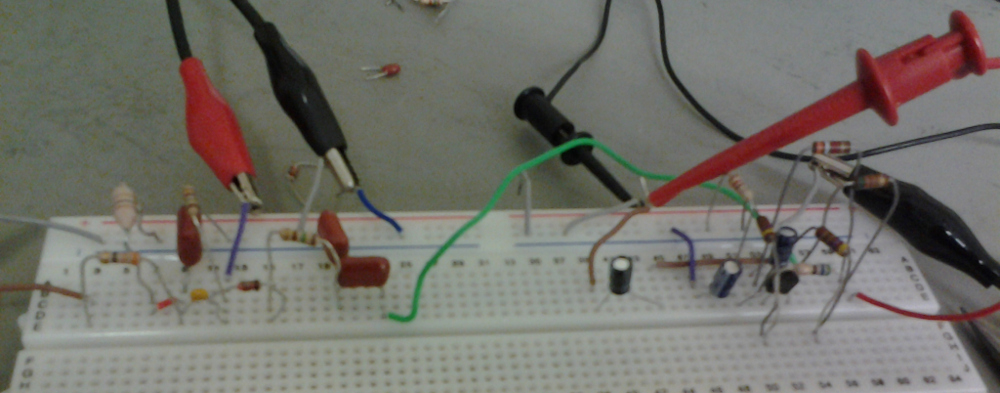
\includegraphics[width=\textwidth]{figures/fullcircuit.jpg}
    \caption{The FM demodulator and the amplifier together. The FM demodulator
    is the circuit on the left and the amplifier is on the right.}
    \label{everything}
\end{figure}

\section{Acknowledgments and Notes}

The lab group that built the FM demodulator and amplifier also consisted of
Leonardo Sattler Cassar\'{a} and David Galbraith. The code used to generate the
plots found in this document can be found on Github at 
https://github.com/isaacdomagalski/astro121-radio-lab/ \cite{Github}.

\newpage
\bibliographystyle{unsrt}
\bibliography{reference_list}{}
\end{document}  
